\begin{figure}[h!]
    \centering
    \caption{Effects of \emph{Plan Cuadrante} on Crime Perception in the Municipality and in the Country}
    \label{fig:figureA3}
    \begin{subfigure}{0.495\textwidth}
        \centering
        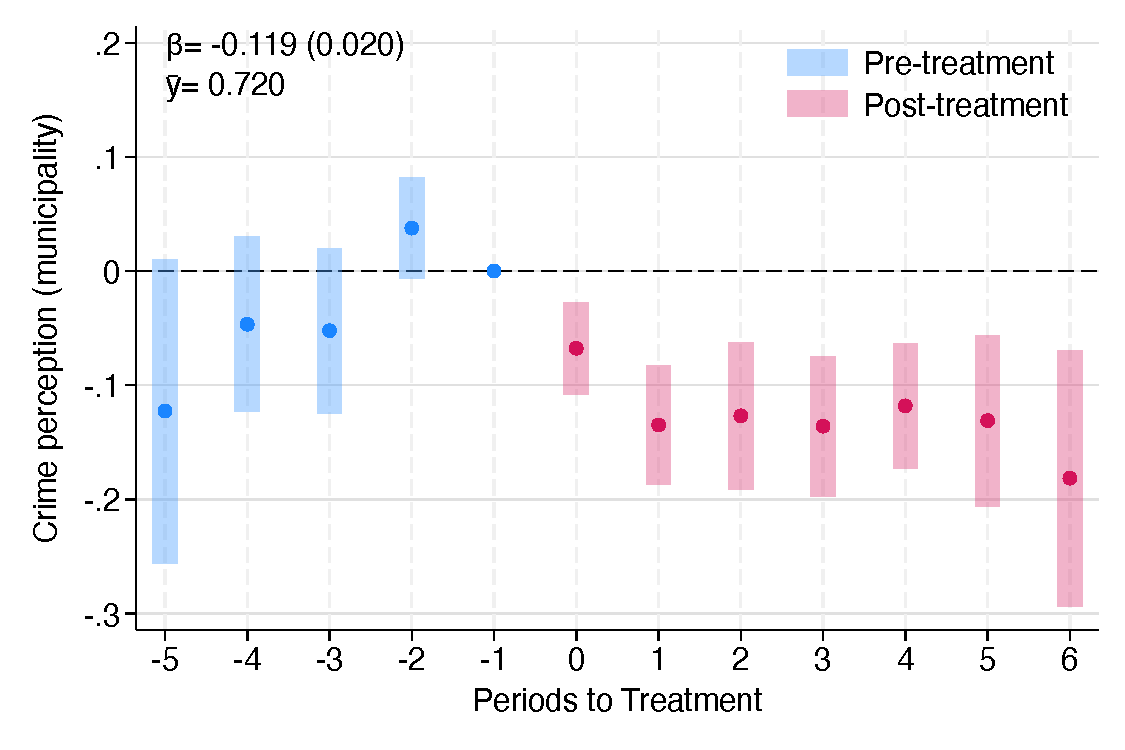
\includegraphics[width=\textwidth]{../manuscript/Graphs/results_perception_municipality.pdf}
        \caption{In the municipality}
    \end{subfigure}%
    ~ 
    \begin{subfigure}{0.495\textwidth}
    \centering
    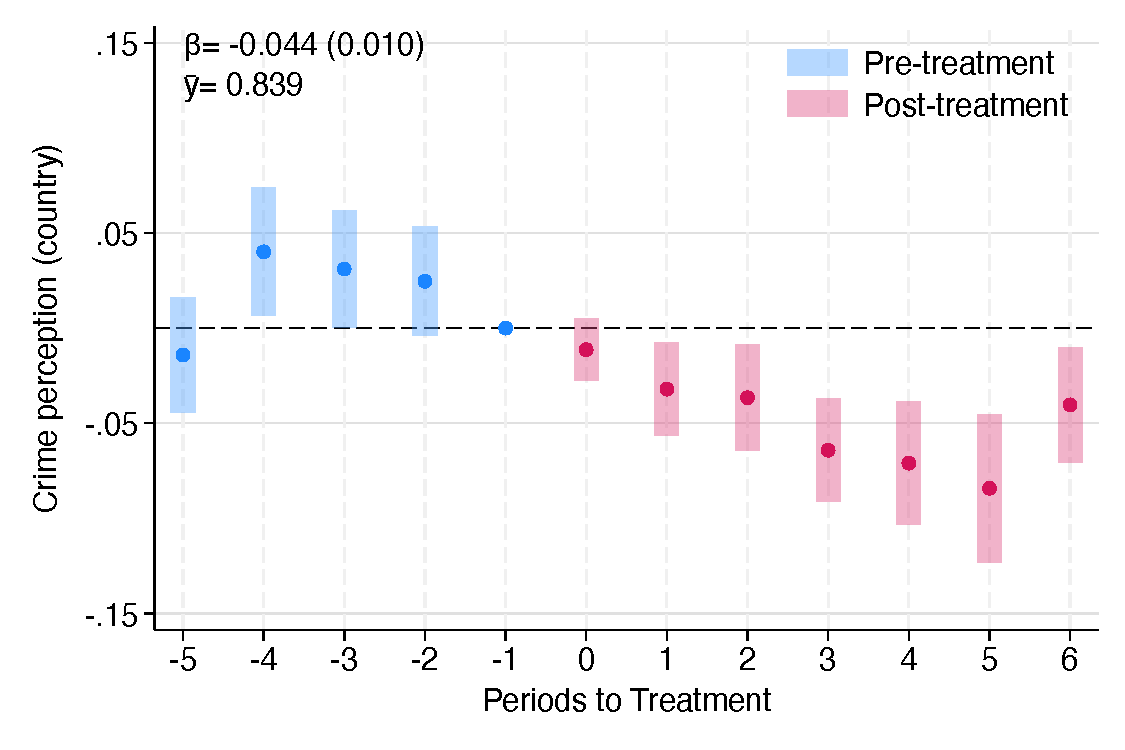
\includegraphics[width=\textwidth]{../manuscript/Graphs/results_perception_country.pdf}
        \caption{In the country}
    \end{subfigure}
    \\[12pt]
    \begin{minipage}{0.99\textwidth}
    \footnotesize Notes: This figure shows the dynamic effects of the \emph{Plan Cuadrante} on the proportion of individuals that perceive an increase in crime in the municipality in the last 12 months (panel a), and on the proportion of individuals that perceive an increase in crime in the country in the last 12 months (panel b). Panel (a) includes 90,696 observations, while panel (b) includes 92,305 observations. The estimation is conducted using the procedure developed in \citet{Callaway} for difference-in-differences with staggered treatment adoption. The dots in the figure represent the estimated coefficients and the bars behind them 95\% confidence intervals. Standard errors are clustered at the municipality level using the wild bootstrapping procedure. The pooled effect and the mean outcome before the introduction of the treatment for every outcome---computed as in Figure \ref{fig:figure02}, using only the pre-treatment observations of treated units---is also presented in each panel.
    \end{minipage}
\end{figure}



 